% Options for packages loaded elsewhere
% Options for packages loaded elsewhere
\PassOptionsToPackage{unicode}{hyperref}
\PassOptionsToPackage{hyphens}{url}
%
\documentclass[
  11pt,
  ignorenonframetext,
  aspectratio=169,
]{beamer}
\newif\ifbibliography
\usepackage{pgfpages}
\setbeamertemplate{caption}[numbered]
\setbeamertemplate{caption label separator}{: }
\setbeamercolor{caption name}{fg=normal text.fg}
\beamertemplatenavigationsymbolsempty
% remove section numbering
\setbeamertemplate{part page}{
  \centering
  \begin{beamercolorbox}[sep=16pt,center]{part title}
    \usebeamerfont{part title}\insertpart\par
  \end{beamercolorbox}
}
\setbeamertemplate{section page}{
  \centering
  \begin{beamercolorbox}[sep=12pt,center]{section title}
    \usebeamerfont{section title}\insertsection\par
  \end{beamercolorbox}
}
\setbeamertemplate{subsection page}{
  \centering
  \begin{beamercolorbox}[sep=8pt,center]{subsection title}
    \usebeamerfont{subsection title}\insertsubsection\par
  \end{beamercolorbox}
}
% Prevent slide breaks in the middle of a paragraph
\widowpenalties 1 10000
\raggedbottom
\AtBeginPart{
  \frame{\partpage}
}
\AtBeginSection{
  \ifbibliography
  \else
    \frame{\sectionpage}
  \fi
}
\AtBeginSubsection{
  \frame{\subsectionpage}
}
\usepackage{iftex}
\ifPDFTeX
  \usepackage[T1]{fontenc}
  \usepackage[utf8]{inputenc}
  \usepackage{textcomp} % provide euro and other symbols
\else % if luatex or xetex
  \usepackage{unicode-math} % this also loads fontspec
  \defaultfontfeatures{Scale=MatchLowercase}
  \defaultfontfeatures[\rmfamily]{Ligatures=TeX,Scale=1}
\fi
\usepackage{lmodern}

\usetheme[]{default}
\ifPDFTeX\else
  % xetex/luatex font selection
\fi
% Use upquote if available, for straight quotes in verbatim environments
\IfFileExists{upquote.sty}{\usepackage{upquote}}{}
\IfFileExists{microtype.sty}{% use microtype if available
  \usepackage[]{microtype}
  \UseMicrotypeSet[protrusion]{basicmath} % disable protrusion for tt fonts
}{}
\makeatletter
\@ifundefined{KOMAClassName}{% if non-KOMA class
  \IfFileExists{parskip.sty}{%
    \usepackage{parskip}
  }{% else
    \setlength{\parindent}{0pt}
    \setlength{\parskip}{6pt plus 2pt minus 1pt}}
}{% if KOMA class
  \KOMAoptions{parskip=half}}
\makeatother


\usepackage{longtable,booktabs,array}
\usepackage{calc} % for calculating minipage widths
\usepackage{caption}
% Make caption package work with longtable
\makeatletter
\def\fnum@table{\tablename~\thetable}
\makeatother
\usepackage{graphicx}
\makeatletter
\newsavebox\pandoc@box
\newcommand*\pandocbounded[1]{% scales image to fit in text height/width
  \sbox\pandoc@box{#1}%
  \Gscale@div\@tempa{\textheight}{\dimexpr\ht\pandoc@box+\dp\pandoc@box\relax}%
  \Gscale@div\@tempb{\linewidth}{\wd\pandoc@box}%
  \ifdim\@tempb\p@<\@tempa\p@\let\@tempa\@tempb\fi% select the smaller of both
  \ifdim\@tempa\p@<\p@\scalebox{\@tempa}{\usebox\pandoc@box}%
  \else\usebox{\pandoc@box}%
  \fi%
}
% Set default figure placement to htbp
\def\fps@figure{htbp}
\makeatother





\setlength{\emergencystretch}{3em} % prevent overfull lines

\providecommand{\tightlist}{%
  \setlength{\itemsep}{0pt}\setlength{\parskip}{0pt}}



 


\setbeamertemplate{itemize items}[circle]
\setbeamertemplate{footline}[frame number]
\definecolor{BgColor}{HTML}{FDF6E3}
\definecolor{TextColor}{HTML}{2B2B2B}
\definecolor{Accent}{HTML}{2E6F95}
\setbeamercolor{background canvas}{bg=BgColor}
\setbeamercolor{normal text}{fg=TextColor}
\setbeamercolor{structure}{fg=Accent}
\usebeamercolor[fg]{normal text}
\usepackage{booktabs}
\usepackage{array}
\usepackage{graphicx}
\usepackage{adjustbox}
\makeatletter
\@ifpackageloaded{caption}{}{\usepackage{caption}}
\AtBeginDocument{%
\ifdefined\contentsname
  \renewcommand*\contentsname{Table of contents}
\else
  \newcommand\contentsname{Table of contents}
\fi
\ifdefined\listfigurename
  \renewcommand*\listfigurename{List of Figures}
\else
  \newcommand\listfigurename{List of Figures}
\fi
\ifdefined\listtablename
  \renewcommand*\listtablename{List of Tables}
\else
  \newcommand\listtablename{List of Tables}
\fi
\ifdefined\figurename
  \renewcommand*\figurename{Figure}
\else
  \newcommand\figurename{Figure}
\fi
\ifdefined\tablename
  \renewcommand*\tablename{Table}
\else
  \newcommand\tablename{Table}
\fi
}
\@ifpackageloaded{float}{}{\usepackage{float}}
\floatstyle{ruled}
\@ifundefined{c@chapter}{\newfloat{codelisting}{h}{lop}}{\newfloat{codelisting}{h}{lop}[chapter]}
\floatname{codelisting}{Listing}
\newcommand*\listoflistings{\listof{codelisting}{List of Listings}}
\makeatother
\makeatletter
\makeatother
\makeatletter
\@ifpackageloaded{caption}{}{\usepackage{caption}}
\@ifpackageloaded{subcaption}{}{\usepackage{subcaption}}
\makeatother

\usepackage{bookmark}
\IfFileExists{xurl.sty}{\usepackage{xurl}}{} % add URL line breaks if available
\urlstyle{same}
\hypersetup{
  pdftitle={Pricing American Put Options with Least-Squares Monte Carlo},
  pdfauthor={Ethan Yao},
  hidelinks,
  pdfcreator={LaTeX via pandoc}}


\title{Pricing American Put Options with Least-Squares Monte Carlo}
\subtitle{Longstaff--Schwartz vs.~Tsitsiklis--Van Roy under a shared
benchmark design}
\author{Ethan Yao}
\date{}

\begin{document}
\frame{\titlepage}


\begin{frame}{From European to American: what changes?}
\phantomsection\label{from-european-to-american-what-changes}
A European option can only be exercised at maturity

Its value depends on a single terminal payoff expectation

An American option can be exercised before maturity

Valuation therefore becomes both:

\begin{itemize}
\tightlist
\item
  a pricing problem
\item
  a decision problem
\end{itemize}
\end{frame}

\begin{frame}{American put pricing as an optimal stopping problem}
\phantomsection\label{american-put-pricing-as-an-optimal-stopping-problem}
We consider a vanilla American put with strike \(K\) and maturity \(T\)

Under the risk-neutral measure, the holder chooses an admissible
stopping time \(\tau\)

The time-0 value is

\[
V_0=\sup_{\tau\in\mathcal T}\mathbb E^{\mathbb Q}\left[e^{-r\tau}(K-S_\tau)^+\right]
\]

American option pricing is therefore an optimal stopping problem
\end{frame}

\begin{frame}{Bellman recursion: exercise vs continuation}
\phantomsection\label{bellman-recursion-exercise-vs-continuation}
At each exercise date, the option value satisfies

\[
V_i(S_{t_i})=\max\{h(S_{t_i}),C_i(S_{t_i})\}
\]

where

\[
h(S_{t_i})=(K-S_{t_i})^+
\]

and

\[
C_i(S_{t_i})=\mathbb E^{\mathbb Q}\left[e^{-r\Delta t}V_{i+1}(S_{t_{i+1}})\mid S_{t_i}\right]
\]

\begin{itemize}
\tightlist
\item
  The holder compares immediate exercise with continuation at each date
\end{itemize}
\end{frame}

\begin{frame}{What exactly is difficult to compute?}
\phantomsection\label{what-exactly-is-difficult-to-compute}
\begin{itemize}
\item
  The intrinsic value is easy to compute
\item
  The main difficulty is the continuation value
\item
  It is an unknown conditional expectation inside a backward recursion
\item
  This is the computational issue that motivates the methods in the rest
  of the presentation
\end{itemize}
\end{frame}

\begin{frame}{Why this project matters}
\phantomsection\label{why-this-project-matters}
American option pricing is an \textbf{optimal stopping} problem. Need
both:

\begin{itemize}
\tightlist
\item
  a price,
\item
  an exercise rule.
\end{itemize}

Direct trees / PDE methods work well in \textbf{simple 1D settings}.

Richer contracts quickly create problems with:

\begin{itemize}
\tightlist
\item
  larger state spaces,
\item
  path dependence,
\item
  changed dynamics.
\end{itemize}

This project studies two regression-based simulation methods under
\textbf{one common design}.

\textbf{Goal:} compare methodology, not mismatched case studies.
\end{frame}

\begin{frame}{Longstaff--Schwartz Paper Walkthrough}
\phantomsection\label{longstaffschwartz-paper-walkthrough}
Simulates risk-neutral paths and works backward from maturity

Estimates continuation values by least-squares regression

Regression target: discounted \textbf{realized future cash flows}

Exercises when intrinsic value exceeds fitted continuation value

Usually regresses only on \textbf{in-the-money} paths
\end{frame}

\begin{frame}{Tsitsiklis--Van Roy Paper Walkthrough}
\phantomsection\label{tsitsiklisvan-roy-paper-walkthrough}
Treats the problem as approximate dynamic programming

Starts from the Bellman recursion and moves backward recursively

Approximates the value / continuation function with basis functions

Regression target: discounted \textbf{next-step estimated values}

Emphasizes approximation error and recursive stability
\end{frame}

\begin{frame}{Methods compared (Josh)}
\phantomsection\label{methods-compared-josh}
\begin{columns}[T]
\begin{column}{0.5\linewidth}
\textbf{Longstaff--Schwartz (LSM)}

\begin{itemize}
\tightlist
\item
  Regress \textbf{discounted realized future cash flows}
\item
  Builds a stopping rule from estimated continuation values
\item
  Main practical pricing method in this project
\end{itemize}
\end{column}

\begin{column}{0.5\linewidth}
\textbf{Tsitsiklis--Van Roy (TVR)}

\begin{itemize}
\tightlist
\item
  Regress \textbf{discounted next-step estimated values}
\item
  Fitted value iteration / approximate dynamic programming
\item
  Matched comparator under the same testbeds
\end{itemize}
\end{column}
\end{columns}

\[
V_i(s)=\max\{h(s),\;C_i(s)\}
\]

\textbf{Key difference:} same Bellman problem, different recursion
target.
\end{frame}

\begin{frame}{Basis functions: how each method implements its regression
(R.B)}
\phantomsection\label{basis-functions-how-each-method-implements-its-regression-r.b}
\begin{columns}[T]
\begin{column}{0.5\linewidth}
\textbf{Longstaff--Schwartz}

Approximates the \textbf{continuation value} \(C_i(S_{t_i})\) using
weighted Laguerre polynomials in normalised spot \(X = S_t/K\):

\[L_0(X) = e^{-X/2}\] \[L_1(X) = e^{-X/2}(1-X)\]
\[L_2(X) = e^{-X/2}(1 - 2X + X^2/2)\]

\begin{itemize}
\tightlist
\item
  Applied to \textbf{in-the-money paths only}
\item
  Regression target: \textbf{realized future cash flows}
\end{itemize}
\end{column}

\begin{column}{0.5\linewidth}
\textbf{Tsitsiklis--Van Roy}

Approximates the \textbf{value function}
\(\tilde{Q}(x,r) = \sum_k r_k \phi_k(x)\) using polynomial basis. What
matters is the best approximation error:

\[\epsilon_n^* = \min_r \|\Phi r - Q_n\|_{\pi_n}\]

\begin{itemize}
\tightlist
\item
  Applied to \textbf{all paths}
\item
  Regression target: \textbf{discounted next-step value estimate}
\end{itemize}
\end{column}
\end{columns}

\textbf{Key difference:} LSM uses realized data; TVR carries forward
fitted estimates. Larger \(\epsilon_n^*\) \(\Rightarrow\) more error
accumulation backward through time.
\end{frame}

\begin{frame}{Experimental Design: one benchmark layer, two extensions}
\phantomsection\label{experimental-design-one-benchmark-layer-two-extensions}
The project is organized around three shared study layers motivated by
corresponding examples in Longstaff--Schwartz paper.

\textbf{Main validation layer:} Vanilla American put under risk-neutral
GBM

\textbf{Shared inputs:}

\begin{itemize}
\tightlist
\item
  \(K=40\), \(r=0.06\)
\item
  \(S_0\in\{36,38,40,42,44\}\)
\item
  \(\sigma\in\{0.20,0.40\}\)
\item
  \(T\in\{1,2\}\)
\item
  50 exercise dates / year
\item
  100,000 paths (50,000 base + 50,000 antithetic)
\end{itemize}

\textbf{Extensions:}

\begin{itemize}
\tightlist
\item
  \textbf{Asian-style:} richer state vector \((S_t,A_t)\)
\item
  \textbf{Jump-style:} changed simulator dynamics
\end{itemize}
\end{frame}

\begin{frame}{Benchmark hierarchy and implementation workflow}
\phantomsection\label{benchmark-hierarchy-and-implementation-workflow}
\[
\text{European BS lower reference}
\rightarrow
\text{Direct American benchmarks (FD, CRR)}
\rightarrow
\] \[
\text{Longstaff / TVR}
\rightarrow
\text{Robustness + extensions}
\]

\begin{block}{Black--Scholes European Benchmark (Lower Reference)}
\phantomsection\label{blackscholes-european-benchmark-lower-reference}
The Black--Scholes European put provides a strict theoretical floor for
the American option, as a non-dividend-paying American put cannot be
worth less than its European equivalent. For spot \(S_0\), strike \(K\),
volatility \(\sigma\), risk-free rate \(r\), and maturity \(T\), the
European price is: \[
P_{\text{Euro}} = K e^{-rT} N(-d_2) - S_0 N(-d_1),
\] where \[
d_1 = \frac{\ln(S_0/K) + \left(r + \tfrac{1}{2}\sigma^2\right)T}{\sigma \sqrt{T}},
\qquad
d_2 = d_1 - \sigma \sqrt{T}.
\] This serves as a lower reference to quantify the early-exercise
premium (\(P_{\text{American}} - P_{\text{Euro}}\)), rather than as the
primary benchmark itself.
\end{block}
\end{frame}

\begin{frame}{Implicit Finite-Difference Benchmark (Primary Reference)}
\phantomsection\label{implicit-finite-difference-benchmark-primary-reference}
The main direct benchmark is an implicit finite-difference solver, which
directly evaluates the one-dimensional early-exercise problem on a
discrete grid in stock price and time. The American put value \(V(S,t)\)
satisfies the Black--Scholes PDE in the continuation region: \[
\frac{\partial V}{\partial t} + \frac{1}{2}\sigma^2 S^2 \frac{\partial^2 V}{\partial S^2} + rS \frac{\partial V}{\partial S} - rV = 0,
\] subject to the terminal payoff \(V(S,T) = (K-S)^+\) and the
early-exercise constraint \(V(S,t) \ge (K-S)^+\). The spatial and time
derivatives are discretized to produce a linear system. Following the
backward step, the numerical value is projected onto the intrinsic
value: \[
V_i^{n} = \max \bigl(V_i^{n,\text{cont}}, K-S_i\bigr),
\] where \(V_i^{n,\text{cont}}\) is the continuation value at node
\((S_i,t_n)\).
\end{frame}

\begin{frame}{CRR Binomial Tree Benchmark (Auxiliary Check)}
\phantomsection\label{crr-binomial-tree-benchmark-auxiliary-check}
A Cox--Ross--Rubinstein (CRR) tree is included to ensure the internal
coherence of the direct American benchmark layer. With time steps
\(\Delta t = T/N\), the stock moves are defined by
\(u = e^{\sigma \sqrt{\Delta t}}\) and \(d = 1/u\), under the
risk-neutral probability \(p = \frac{e^{r\Delta t} - d}{u-d}\). The tree
evaluates the terminal payoff \(V_N(j) = (K - S_N(j))^+\) and is rolled
backward via: \[
C_n(j) = e^{-r\Delta t}\bigl(p V_{n+1}(j+1) + (1-p)V_{n+1}(j)\bigr),
\] enforcing the early-exercise condition
\(V_n(j) = \max \bigl((K-S_n(j))^+, C_n(j)\bigr)\) at each node.
\end{frame}

\begin{frame}{}
\phantomsection\label{section}
Shared pieces wherever possible:

\begin{itemize}
\tightlist
\item
  simulator,
\item
  basis construction,
\item
  benchmark logic.
\end{itemize}

Different pieces:

\begin{itemize}
\tightlist
\item
  \textbf{LSM:} continuation-cash-flow regression,
\item
  \textbf{TVR:} fitted value recursion.
\end{itemize}

In both methods, the fitted policy is then evaluated on fresh paths.

\textbf{Why this matters:} same environment, different recursion logic.
\end{frame}

\begin{frame}{Vanilla benchmark: methods are sensible, but not
interchangeable}
\phantomsection\label{vanilla-benchmark-methods-are-sensible-but-not-interchangeable}
\begin{table}
\small
\centering
\begin{tabular}{lrrrr}
\toprule
Case & FD & LSMC (OOS) & TVR (OOS) & Pattern \\
\midrule
$S_0=36,\ \sigma=0.2,\ T=1$ & 4.463 & 4.206 & 4.385 & TVR closer \\
$S_0=40,\ \sigma=0.2,\ T=1$ & 2.299 & 2.444 & 2.278 & LSM high, TVR close \\
$S_0=40,\ \sigma=0.2,\ T=2$ & 2.873 & 2.727 & 2.829 & both reasonable \\
$S_0=40,\ \sigma=0.4,\ T=2$ & 6.897 & 6.971 & 6.859 & both close \\
$S_0=44,\ \sigma=0.4,\ T=1$ & 3.924 & 4.132 & 3.838 & LSM high, TVR low \\
\bottomrule
\end{tabular}%
\caption{Partial Results of Vanilla American put pricing comparison under different spot, volatility, and maturity settings.}
\end{table}

\begin{itemize}
\tightlist
\item
  Both methods produce \textbf{economically sensible American put
  values}.
\item
  LSM can price \textbf{above or below} the FD benchmark.
\item
  TVR tends to stay \textbf{near FD} and often slightly \textbf{below}
  it.
\end{itemize}

\textbf{Takeaway:} differences are methodological, not noise from
different setups.
\end{frame}

\begin{frame}{Vanilla visuals: benchmark alignment}
\phantomsection\label{vanilla-visuals-benchmark-alignment}
\begin{columns}[T]
\begin{column}{0.5\linewidth}
\begin{figure}[H]

{\centering 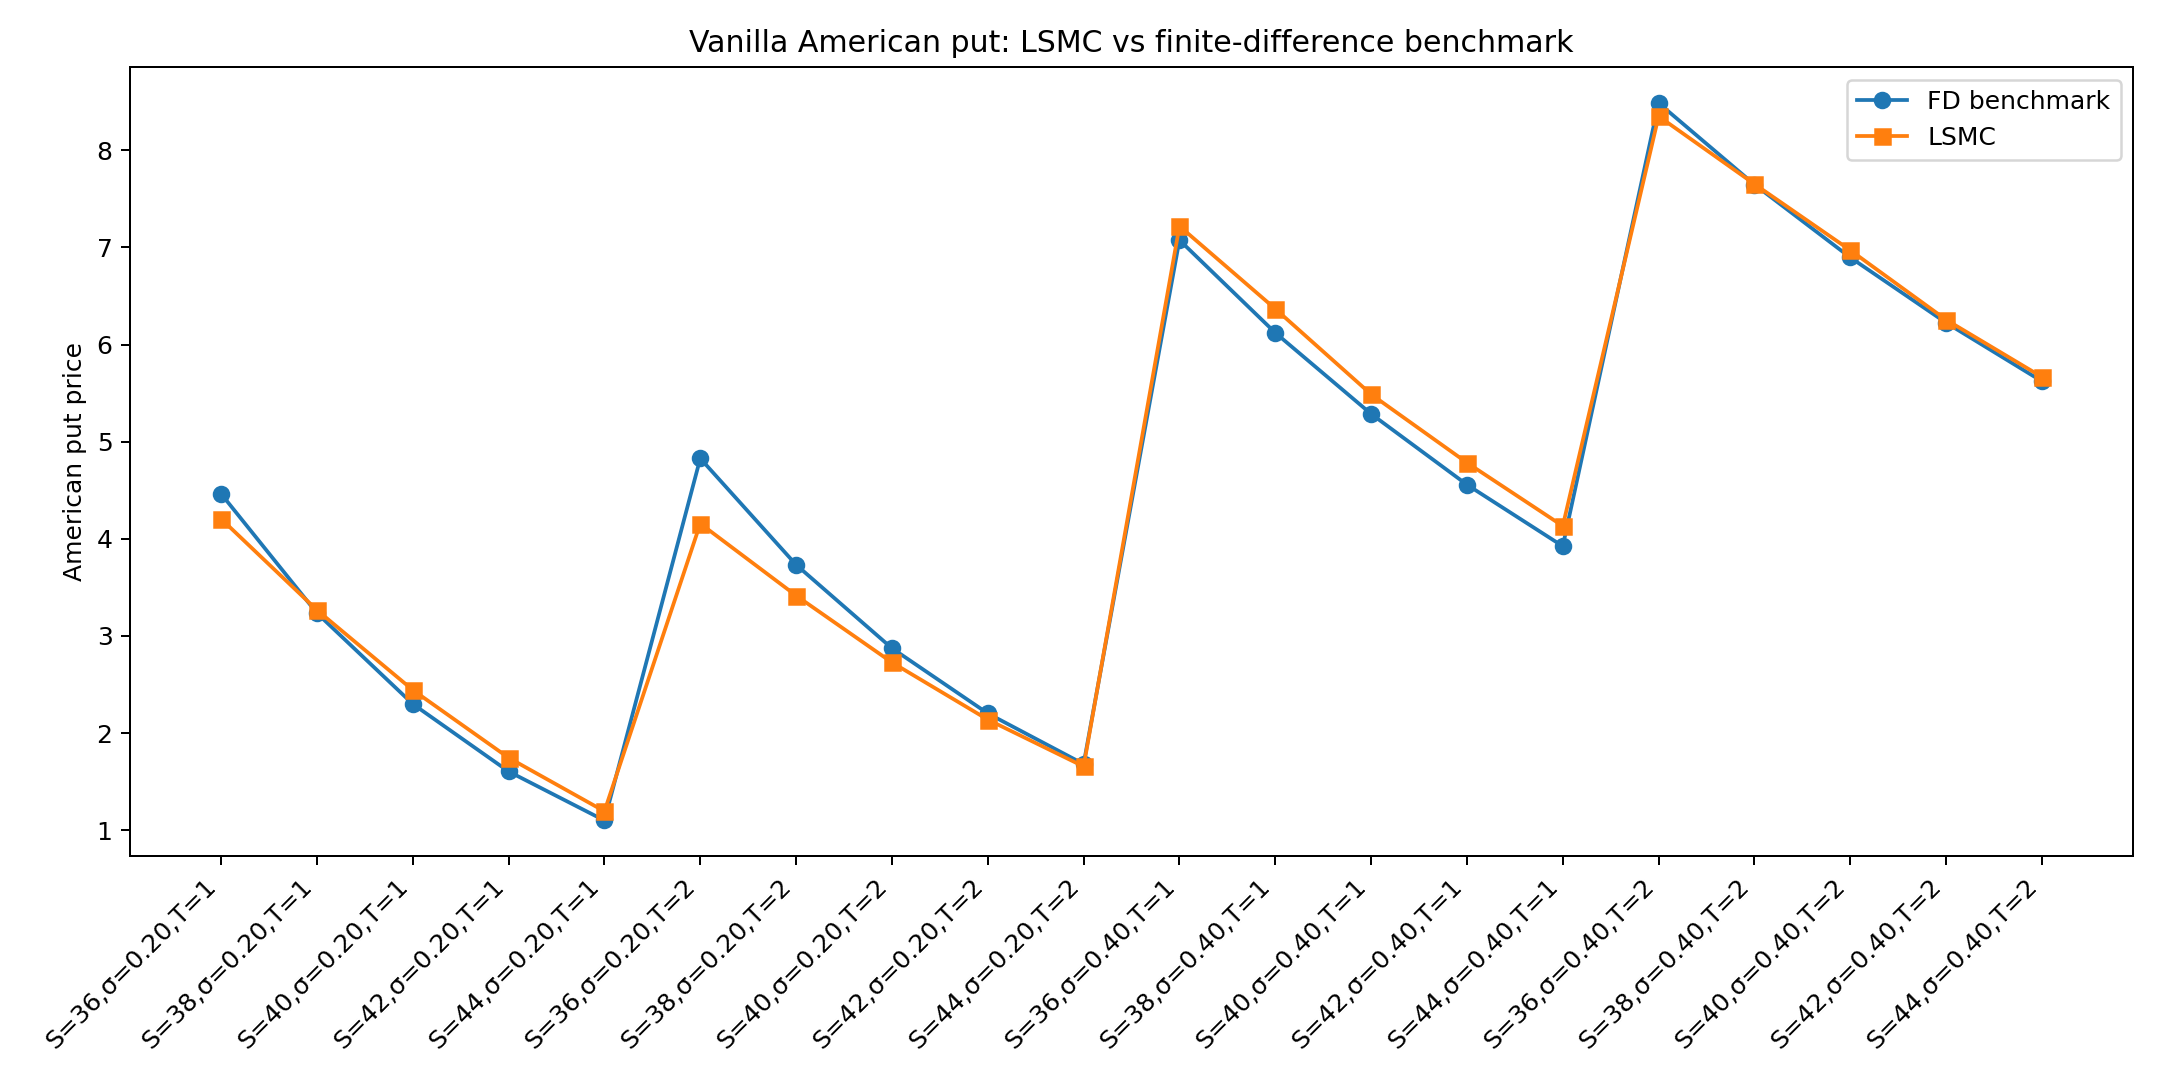
\includegraphics[width=1\linewidth,height=\textheight,keepaspectratio]{../visuals/longstaff_vanilla_benchmark_comparison.png}

}

\caption{Longstaff benchmark vs finite difference.}

\end{figure}%

\textbf{LSM:} tighter than same-path pricing, but still case-dependent
around FD.
\end{column}

\begin{column}{0.5\linewidth}
\begin{figure}[H]

{\centering 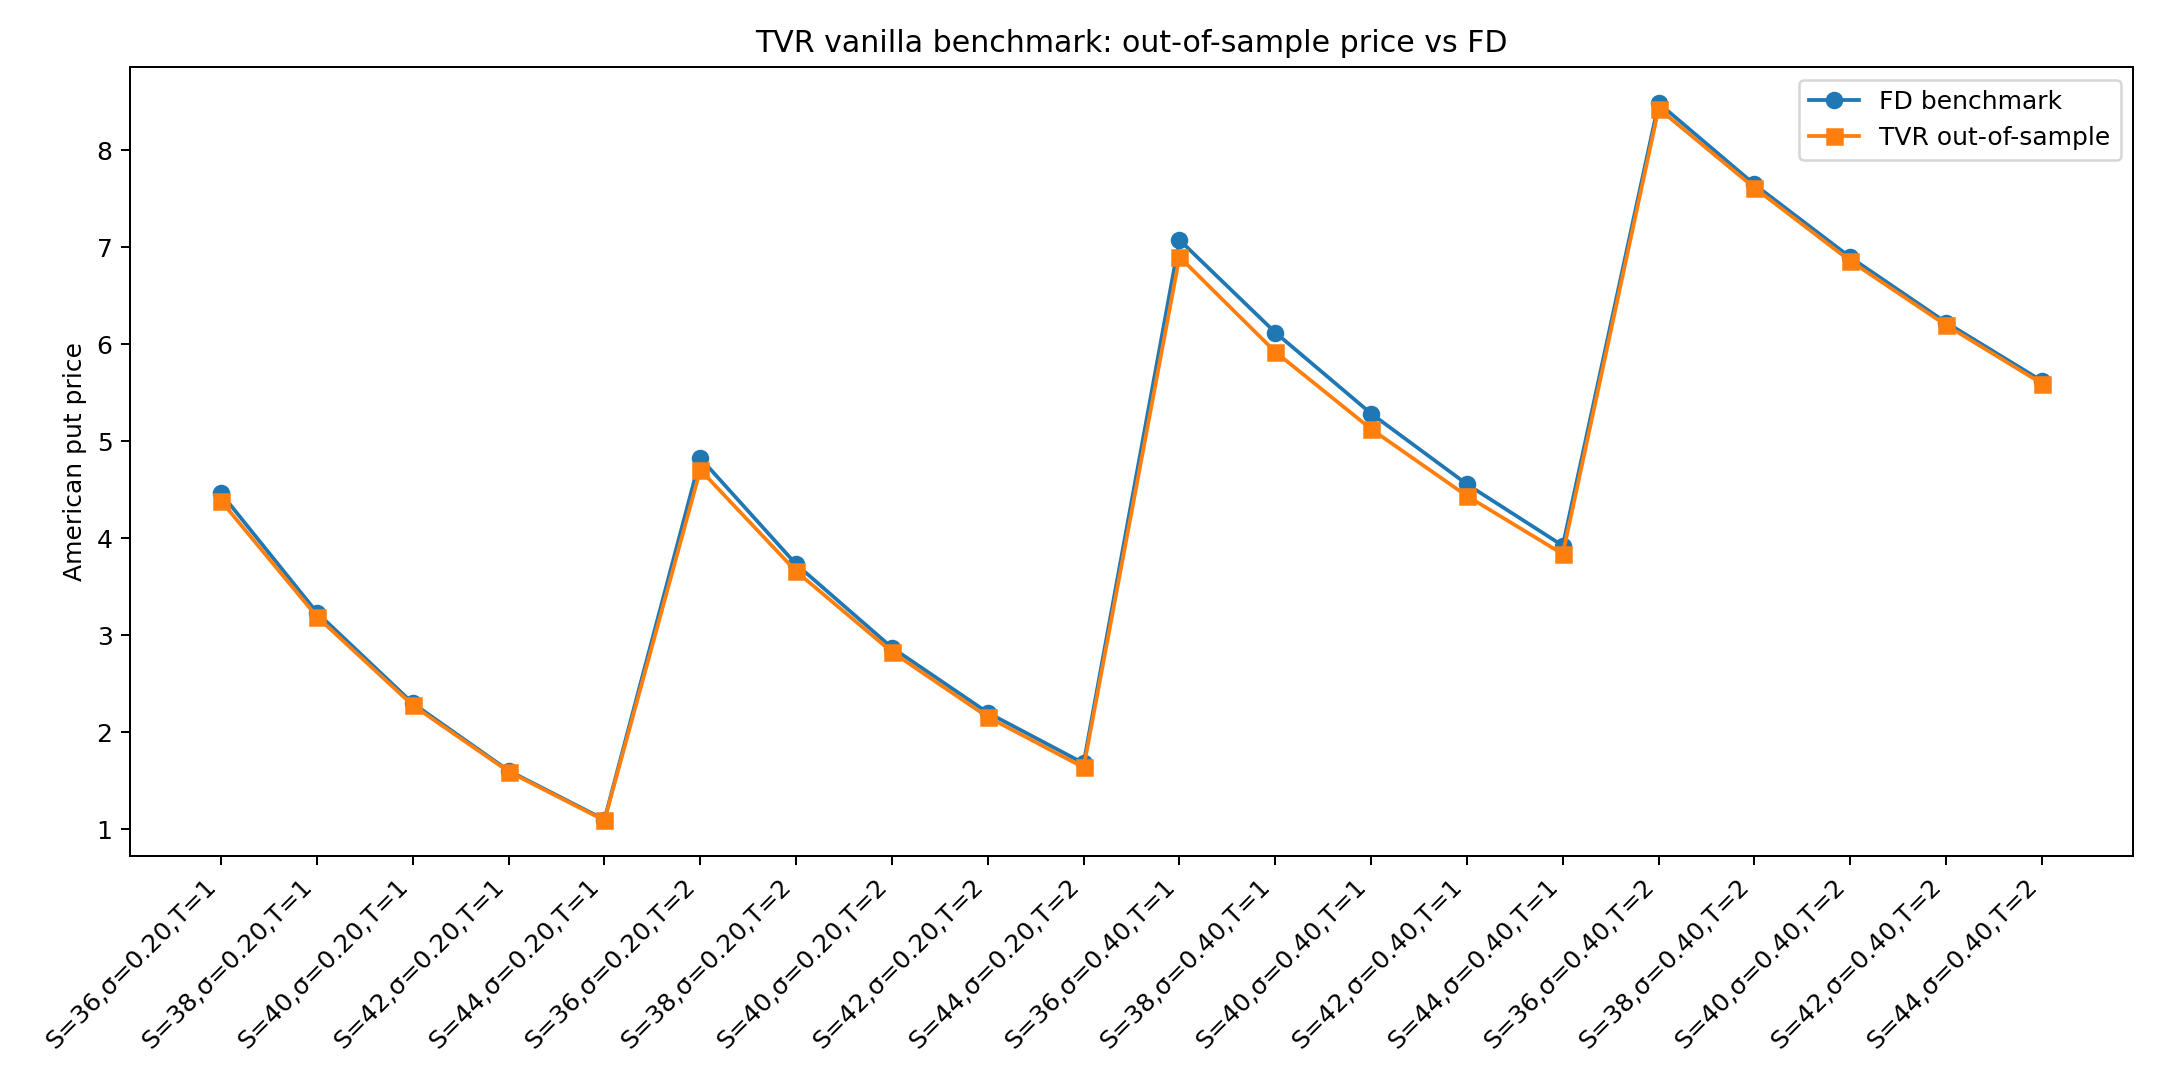
\includegraphics[width=1\linewidth,height=\textheight,keepaspectratio]{../visuals/tvr_vanilla_benchmark_comparison.png}

}

\caption{TVR benchmark vs finite difference.}

\end{figure}%

\textbf{TVR:} clusters more closely around FD across the shared grid.
\end{column}
\end{columns}
\end{frame}

\begin{frame}{Validation matters: same-path optimism is mainly a
Longstaff issue}
\phantomsection\label{validation-matters-same-path-optimism-is-mainly-a-longstaff-issue}
\begin{table}
\small
\centering
\begin{tabular}{lrrr}
\toprule
Representative case & In-sample & Out-of-sample & Fit - Eval \\
\midrule
LSM: $S_0=36,\ \sigma=0.2,\ T=1$ & 4.452 & 4.206 & 0.247 \\
LSM: $S_0=40,\ \sigma=0.2,\ T=2$ & 3.060 & 2.739 & 0.321 \\
LSM: $S_0=40,\ \sigma=0.4,\ T=2$ & 7.810 & 6.956 & 0.854 \\
\midrule
TVR: $S_0=36,\ \sigma=0.2,\ T=1$ & 4.386 & 4.381 & 0.005 \\
TVR: $S_0=40,\ \sigma=0.2,\ T=2$ & 2.804 & 2.817 & -0.014 \\
TVR: $S_0=44,\ \sigma=0.4,\ T=1$ & 3.865 & 3.840 & 0.025 \\
\bottomrule
\end{tabular}%
\end{table}

\begin{itemize}
\tightlist
\item
  LSM shows \textbf{clear same-path optimism}.
\item
  TVR fit/eval gaps are \textbf{much smaller}.
\end{itemize}

\textbf{Takeaway:} out-of-sample policy evaluation is not optional.
\end{frame}

\begin{frame}{Robustness snapshots}
\phantomsection\label{robustness-snapshots}
\begin{table}
\small
\centering
\begin{tabular}{llrr}
\toprule
Test & Case & LSM pattern & TVR pattern \\
\midrule
Paths(25000 \to 200000) & $(40,0.2,1)$ & 2.317 \to 2.447 & 2.270 \to 2.282 \\
Paths(25000 \to 200000) & $(40,0.4,2)$ & 6.935 \to 6.958 & 6.889 \to 6.850 \\
Grid(Ex. Dates/Yr 25 \to 100) & $(40,0.2,1)$ & 2.561 \to 2.344 & 2.295 \to 2.281 \\
Grid(Ex. Dates/Yr 25 \to 100) & $(40,0.4,2)$ & 7.210 \to 6.827 & 6.864 \to 6.819 \\
Basis(2 \to 5) & $(40,0.2,1)$ & 2.385 \to 2.458 & 2.151 \to 2.285 \\
Basis(2 \to 5) & $(40,0.4,2)$ & 6.890 \to 6.992 & 6.466 \to 6.862 \\
\bottomrule
\end{tabular}
\caption{Partial Results of In-sample versus Out-of-sample Policy Valuation for Representative Vanilla American Put Cases}
\end{table}

\begin{itemize}
\tightlist
\item
  LSM is more sensitive to the interaction of fit and stopping-rule
  construction.
\item
  TVR is more constrained by \textbf{under-parameterization} when the
  basis is too small.
\end{itemize}
\end{frame}

\begin{frame}{Robustness: what moves the price?}
\phantomsection\label{robustness-what-moves-the-price}
\begin{columns}[T]
\begin{column}{0.49\linewidth}
\textbf{Longstaff}

\begin{itemize}
\tightlist
\item
  Path count reduces SE, but not monotone benchmark error
\item
  Sensitive to exercise grid
\item
  Sensitive to basis choice
\item
  Seed variation is smaller than the main benchmark gaps
\end{itemize}
\end{column}

\begin{column}{0.49\linewidth}
\textbf{TVR}

\begin{itemize}
\tightlist
\item
  Also benefits from more paths
\item
  More stable across path budgets
\item
  More directional improvement with richer bases
\item
  Still mildly conservative against FD
\end{itemize}
\end{column}
\end{columns}

\textbf{Main message:} price quality depends on more than path count:

\begin{itemize}
\tightlist
\item
  basis design,
\item
  exercise grid,
\item
  validation structure,
\item
  approximation target.
\end{itemize}
\end{frame}

\begin{frame}{Asian-style extension: American--Bermuda--Asian put}
\phantomsection\label{asian-style-extension-americanbermudaasian-put}
The state space is expanded to include both current spot and a running
arithmetic average, with exercise restricted by a lockout period.

Under the risk-neutral measure, the stock follows GBM: \[
dS_t = r S_t dt + \sigma S_t dW_t^{\mathbb Q},
\]

with constant r and \(\sigma\). In the present Asian benchmark, the
contract parameters are set to K = 100, r = 0.06, \(\sigma = 0.20\), T =
2, with a lockout period of 0.25 years and 100 exercise dates per year
in the discrete approximation. The same contract scope is used for both
Longstaff and TVR.
\end{frame}

\begin{frame}{}
\phantomsection\label{section-1}
To reflect the paper's idea that the average starts before valuation, we
use a pre-started running arithmetic average: \[
A_t = \frac{\delta A_0 + \int_0^t S_u,du}{\delta + t},
\qquad \delta = 0.25,
\]

where \(A_0\) is the initial average level specified in the benchmark
grid. In the code, this is the second state variable carried along each
simulated path.

The payoff from immediate exercise at time t is
\(h(S_t,A_t)=(K-A_t)^+,\) so this is an average-based put rather than a
spot-based vanilla put. Exercise is not allowed before the lockout date
\(t_{\mathrm{lock}}=0.25\). The time-zero value is therefore

\[
V_0 = \sup_{\tau \in \mathcal T,\ \tau \ge t_{\mathrm{lock}}}
\mathbb E^{\mathbb Q} \left[e^{-r\tau}(K-A_\tau)^+\right].
\]
\end{frame}

\begin{frame}{}
\phantomsection\label{section-2}
With exercise dates \((0=t_0<t_1<\cdots<t_N=T)\), the discrete-time
Bellman recursion is \[
V_i(s,a)
=
\max\left\{
(K-a)^+,\;
\mathbb{E}^{\mathbb{Q}}\!\left[
e^{-r\Delta t}V_{i+1}(S_{t_{i+1}},A_{t_{i+1}})
\mid S_{t_i}=s,\ A_{t_i}=a
\right]
\right\}.
\]

for dates after the lockout, with terminal condition
\(V_N(s,a)=(K-a)^{+}.\)

\textbf{Purpose:} move from 1D vanilla validation to a richer
continuation problem.
\end{frame}

\begin{frame}{Asian-style results: both methods work, policies differ}
\phantomsection\label{asian-style-results-both-methods-work-policies-differ}
\begin{table}
\small
\centering
\begin{tabular}{lrrrr}
\toprule
Representative case & LSM (OOS) & LSM Fit-Eval & TVR (OOS) & TVR - LSM \\
\midrule
$A_0=90,\ S_0=80$ & 13.777 & 1.016 & 17.498 & 3.720 \\
$A_0=100,\ S_0=100$ & 3.213 & 0.122 & 3.598 & 0.384 \\
$A_0=110,\ S_0=110$ & 1.066 & 0.068 & 1.078 & 0.013 \\
\bottomrule
\end{tabular}
\caption{Partial results on the paper-inspired $(A_0,S_0)$ grid with $K=100$, $r=0.06$, $\sigma=0.2$, $T=2$, lockout $=0.25$, and 100 exercise dates per year.}
\end{table}

\begin{itemize}
\item
  Both methods show the right comparative statics.
\item
  LSM still has \textbf{positive fit-vs-eval gaps}.
\item
  TVR is more \textbf{validation-stable} and often gives \textbf{higher
  values}.
\end{itemize}

\textbf{Interpretation:} multistate comparison only --- not a direct PDE
benchmark exercise.
\end{frame}

\begin{frame}{Among all states the simulation visits at date t, where
does the fitted policy choose to stop rather than continue?}
\phantomsection\label{among-all-states-the-simulation-visits-at-date-t-where-does-the-fitted-policy-choose-to-stop-rather-than-continue}
Snapshot of T = 2, \(A_0=S_0=100\) at t = 1. x-axis = Spot \(S_t\),
y-axis = Average \(A_t\), the color bar is intrinsic value at time t

\begin{columns}[T]
\begin{column}{0.4\linewidth}
\begin{figure}[H]

{\centering 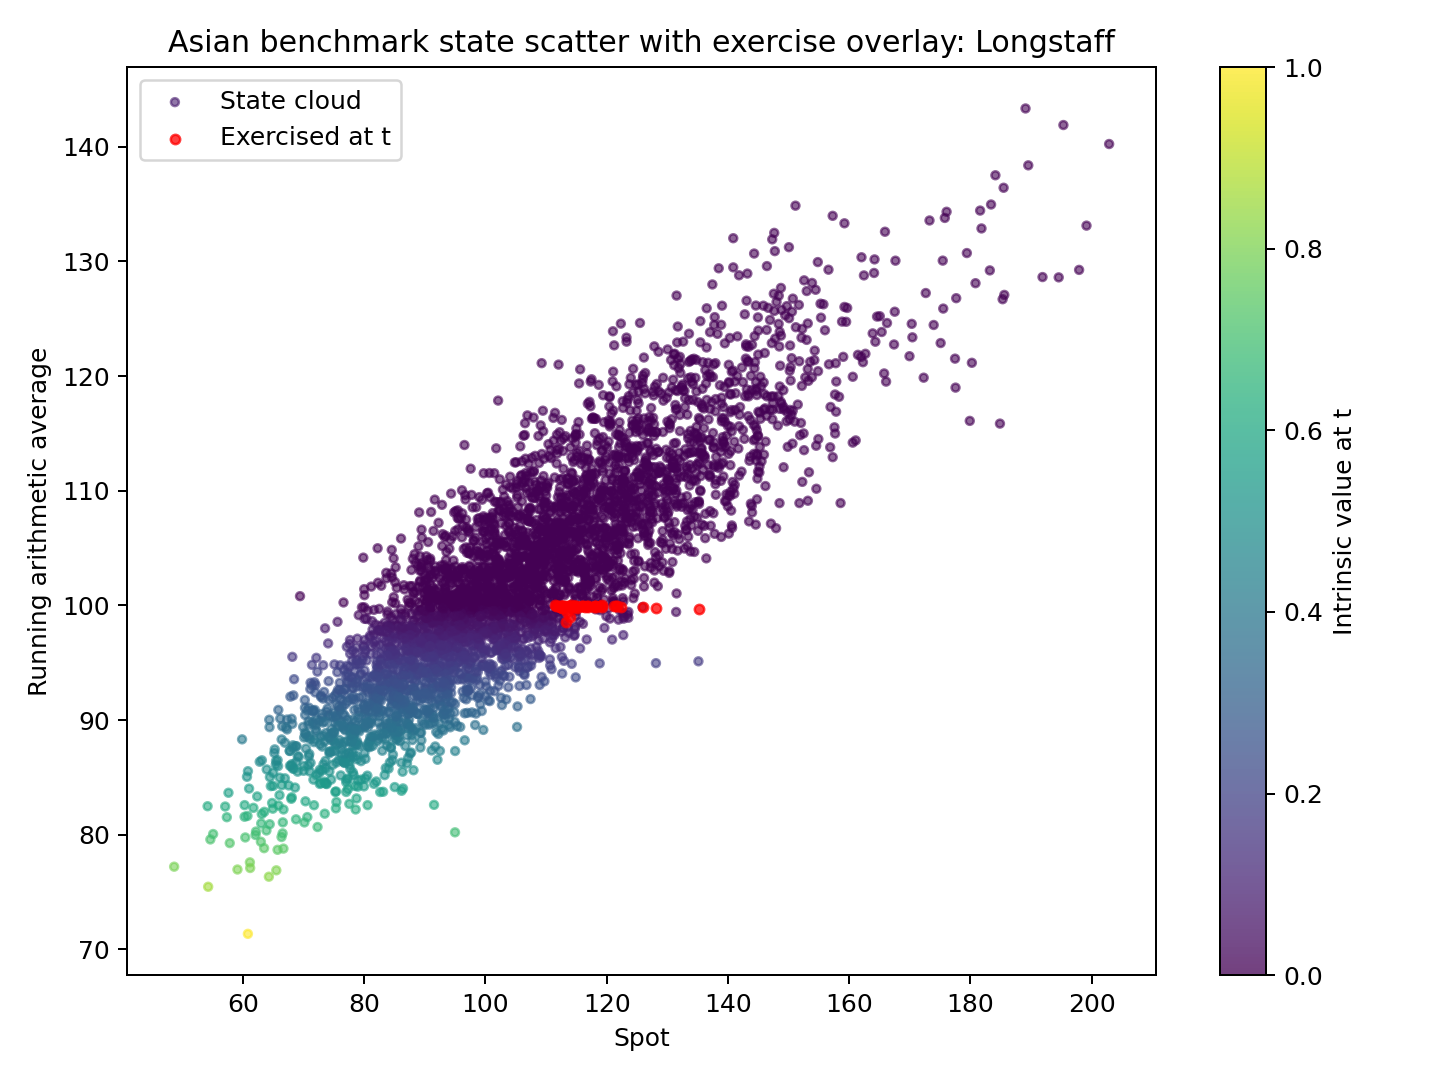
\includegraphics[width=1\linewidth,height=\textheight,keepaspectratio]{../visuals/longstaff_asian_state_scatter.png}

}

\caption{Longstaff Asian state cloud with exercise overlay.}

\end{figure}%

More exercise-prone in borderline states.
\end{column}

\begin{column}{0.4\linewidth}
\begin{figure}[H]

{\centering 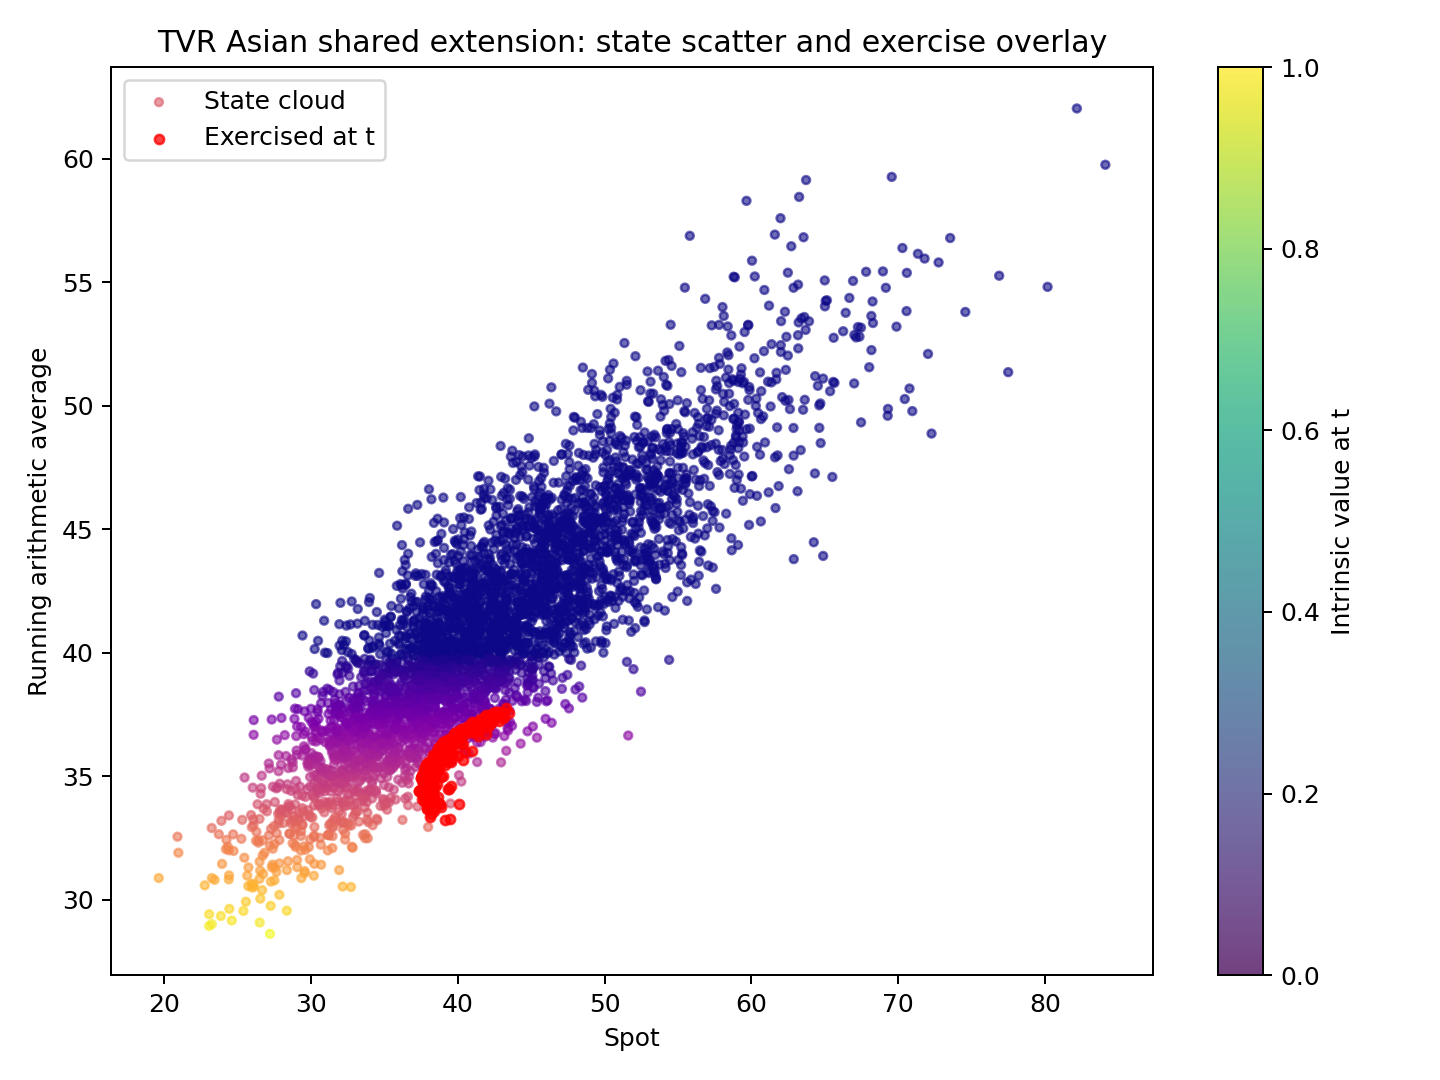
\includegraphics[width=1\linewidth,height=\textheight,keepaspectratio]{../visuals/tvr_asian_state_scatter.png}

}

\caption{TVR Asian state cloud with exercise overlay.}

\end{figure}%

More continuation-oriented
\end{column}
\end{columns}
\end{frame}

\begin{frame}{Jump-style extension: changed-dynamics study}
\phantomsection\label{jump-style-extension-changed-dynamics-study}
The final layer replaces the standard GBM simulator with a stylized
jump-to-ruin process.

Under the risk-neutral measure, we use a stylized jump-to-ruin process
of the form \[
dS_t = (r+\lambda)S_t dt + \sigma S_t dW_t^{\mathbb Q} - S_{t^-} dq_t,
\]

where \(q_t\) is a Poisson process with intensity \(\lambda\). When a
jump occurs, the stock is sent to zero and remains there afterward. The
\(r+\lambda\) drift adjustment is the martingale correction used in the
paper's jump comparison.
\end{frame}

\begin{frame}{}
\phantomsection\label{section-3}
The immediate exercise payoff remains the vanilla American put payoff,
\(h(S_t) = (K-S_t)^+,\) so the time-zero value is \[
V_0 = \sup_{\tau \in \mathcal T}
\mathbb E^{\mathbb Q} \left[e^{-r\tau}(K-S_\tau)^+\right].
\]

With exercise dates \(0=t_0<t_1<\cdots<t_N=T\), the discrete-time
Bellman recursion is \[
V_i(s)=
\max\left\{
(K-s)^+,\;
\mathbb{E}^{\mathbb{Q}}\!\left[
e^{-r\Delta t} V_{i+1}(S_{t_{i+1}})
\,\middle|\, S_{t_i}=s
\right]
\right\}.
\]

We compare two cases with the same strike and maturity, K = 40, r =
0.06, T = 1, using 26 exercise dates per year:

\begin{itemize}
\tightlist
\item
  \textbf{no jump:} \(\lambda=0, \sigma=0.30\)
\item
  \textbf{jump-to-ruin:} \(\lambda=0.05, \sigma=0.20\).
\end{itemize}

\textbf{Purpose:} test whether both methods remain coherent when
dynamics change.
\end{frame}

\begin{frame}{Jump-style results: changed dynamics, same methodological
contrast}
\phantomsection\label{jump-style-results-changed-dynamics-same-methodological-contrast}
\begin{table}
\small
\centering
\begin{tabular}{lrrrr}
\toprule
Case at $S_0=40$ & American & Euro MC & Premium & Fit-Eval \\
\midrule
LSM no-jump & 4.093 & 3.570 & 0.523 & 0.235 \\
LSM jump-to-ruin & 3.614 & 3.220 & 0.394 & 0.149 \\
TVR no-jump & 3.743 & 3.588 & 0.155 & 0.001 \\
TVR jump-to-ruin & 3.277 & 3.217 & 0.060 & -0.020 \\
\bottomrule
\end{tabular}
\caption{Partial results on the matched jump grid with $K=40$, $r=0.06$, $T=1$, 26 exercise dates per year, and 50{,}000 total paths. The no-jump case uses $\sigma=0.30,\ \lambda=0.00$, while the jump-to-ruin case uses $\sigma=0.20,\ \lambda=0.05$.}
\end{table}

\begin{itemize}
\item
  Across the full jump grid, values fall with spot in both model cases.
\item
  American values remain above European MC values.
\item
  In this matched design, \textbf{jump-to-ruin values are generally
  lower} than no-jump values.
\item
  TVR remains more conservative than LSM.
\end{itemize}
\end{frame}

\begin{frame}{Jump-style visuals: price ranking + exercised-state
summary}
\phantomsection\label{jump-style-visuals-price-ranking-exercised-state-summary}
\begin{columns}[T]
\begin{column}{0.5\linewidth}
\begin{figure}[H]

{\centering 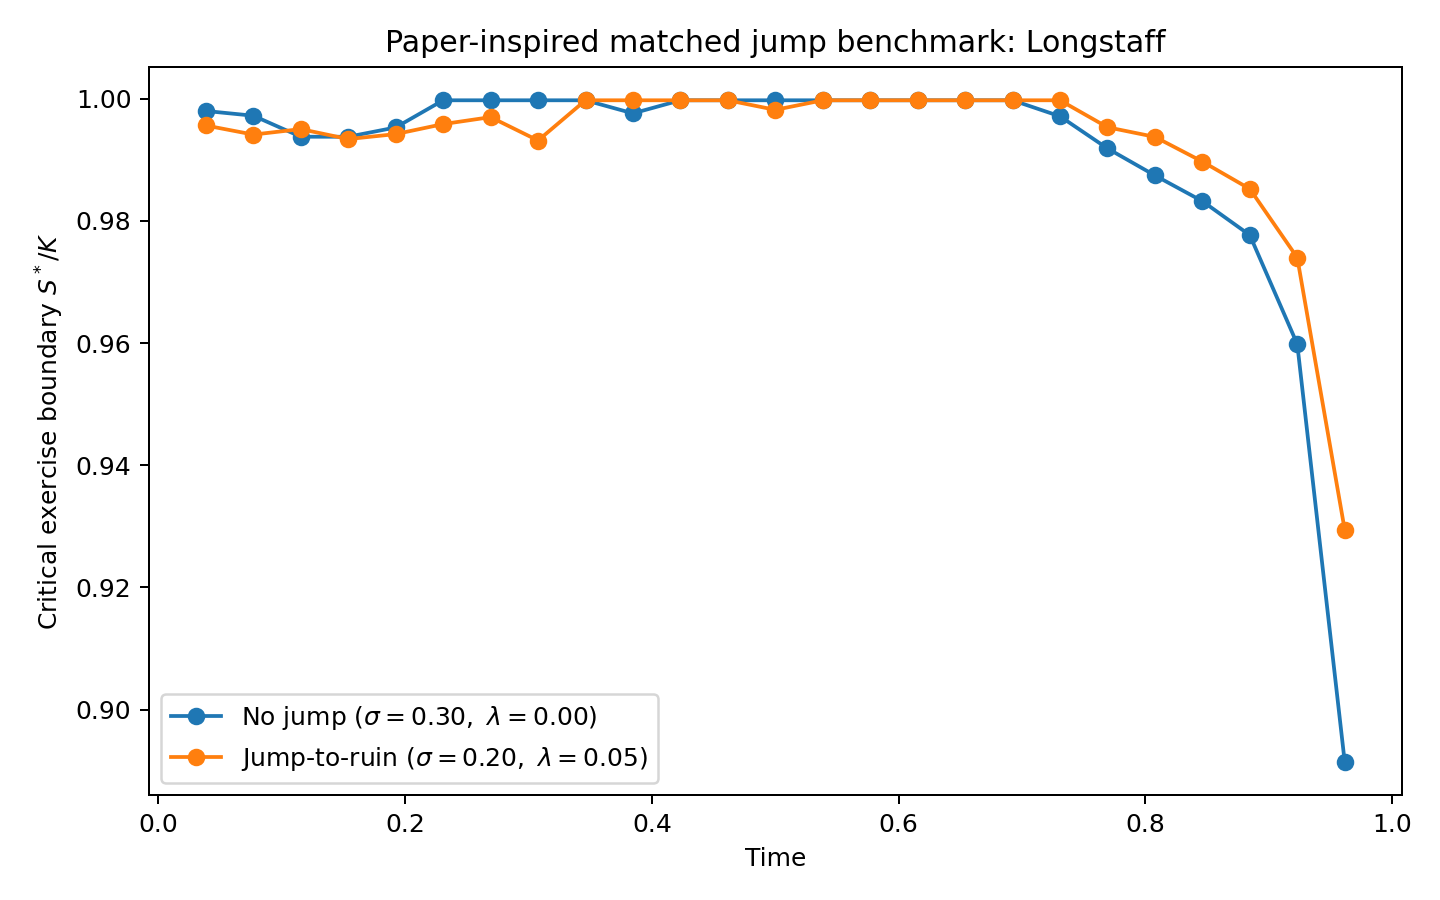
\includegraphics[width=1\linewidth,height=\textheight,keepaspectratio]{../visuals/longstaff_jump_boundary_comparison.png}

}

\caption{Longstaff matched jump extension}

\end{figure}%

\textbf{LSM:} coherent under changed dynamics, but more exercise-prone.
\end{column}

\begin{column}{0.5\linewidth}
\begin{figure}[H]

{\centering 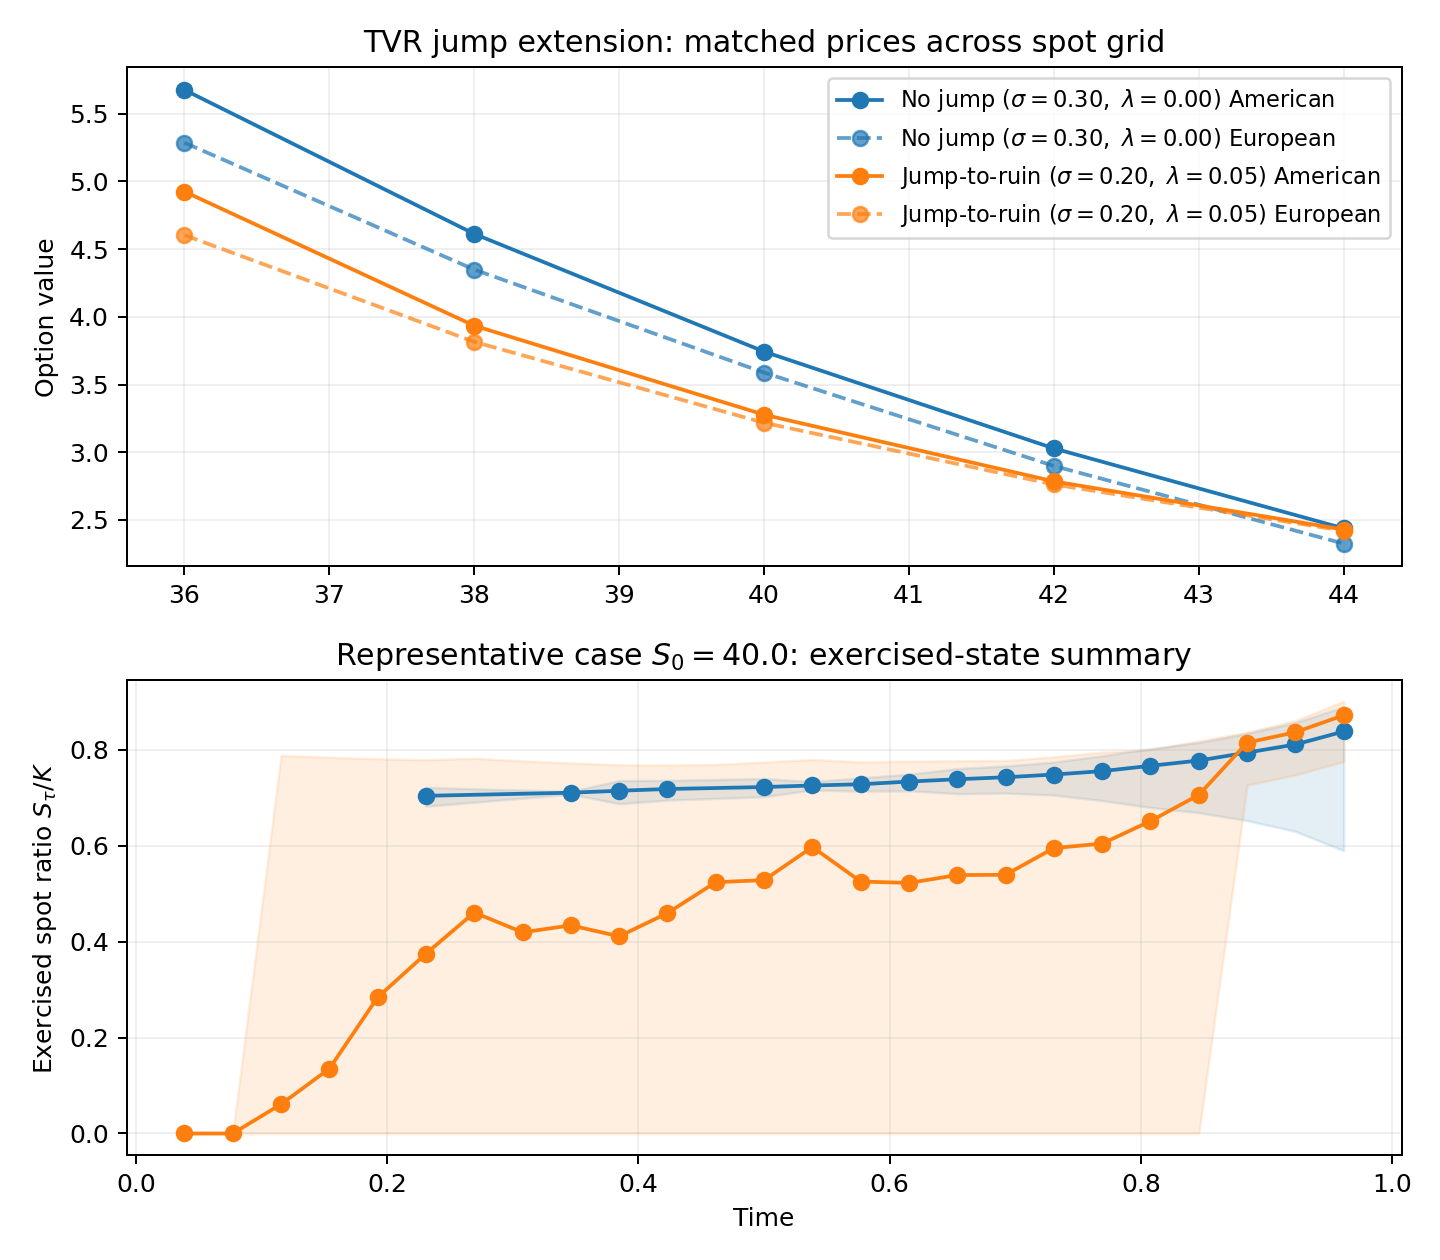
\includegraphics[width=1\linewidth,height=\textheight,keepaspectratio]{../visuals/tvr_jump_boundary_comparison.png}

}

\caption{TVR matched jump extension}

\end{figure}%

\textbf{TVR:} same ranking, more selective exercise; smaller fit/eval
gap
\end{column}
\end{columns}
\end{frame}

\begin{frame}{Direct Longstaff vs TVR comparison (R.B)}
\phantomsection\label{direct-longstaff-vs-tvr-comparison-r.b}
\begin{columns}[T]
\begin{column}{0.5\linewidth}
\textbf{Longstaff--Schwartz}

\begin{itemize}
\item
  More directly tied to stopping-rule construction
\item
  Strong practical simulation method
\item
  More sensitive to:

  \begin{itemize}
  \tightlist
  \item
    fit/eval separation,
  \item
    basis design,
  \item
    exercise-grid design
  \end{itemize}
\item
  Can look optimistic if only same-path values are reported
\end{itemize}
\end{column}

\begin{column}{0.5\linewidth}
\textbf{Tsitsiklis--Van Roy}

\begin{itemize}
\tightlist
\item
  More naturally read as fitted value iteration
\item
  More stable under matched out-of-sample evaluation
\item
  Often mildly conservative in benchmark alignment
\end{itemize}
\end{column}
\end{columns}

\textbf{Bottom line:} same optimal stopping problem, different numerical
behavior.
\end{frame}

\begin{frame}{Convergence theory: why the two methods behave differently
(R.B)}
\phantomsection\label{convergence-theory-why-the-two-methods-behave-differently-r.b}
\textbf{LSM: Proposition 1 (downward bias)}

\[V(X) \geq \lim_{N\to\infty} \frac{1}{N}\sum_{i=1}^N \text{LSM}(\omega_i; M, K)\]

LSM produces a stopping rule --- asymptotically never overstates true
value. But in finite samples with a finite basis, prices can sit above
or below a numerical benchmark. The large fit/eval gaps in our results
confirm that same-path evaluation overstates performance.
\end{frame}

\begin{frame}{}
\phantomsection\label{section-4}
\textbf{TVR: Theorem 1 (bounded error under trajectory sampling)}

\[\tilde{e}_n^2 \leq \alpha^2 \tilde{e}_{n+1}^2 + (\epsilon_n^*)^2\]

If states are sampled from the risk-neutral trajectory distribution,
error is bounded:

\[\tilde{e}_n \leq \frac{\epsilon}{\sqrt{2(1-\alpha^2)}} \quad \textbf{independent of } N\]

Without trajectory sampling, errors grow \textbf{exponentially} with
horizon.
\end{frame}

\begin{frame}{}
\phantomsection\label{section-5}
\textbf{TVR: Theorem 2 (almost sure convergence)}

\[\hat{r}_n(m) \xrightarrow{a.s.} r_n \quad \text{as } m \to \infty\]

Sample-based regression converges to the idealised algorithm as paths
grow.

\textbf{This explains our results:} TVR's small fit/eval gaps reflect
bounded error accumulation. LSM's large gaps reflect in-sample optimism
that out-of-sample evaluation corrects. Our basis sensitivity tables
show \(\epsilon_n^*\) shrinking as basis grows --- exactly as Theorem 1
predicts.
\end{frame}

\begin{frame}{Implementation Scope and Claims}
\phantomsection\label{implementation-scope-and-claims}
The project does \textbf{not} claim strict numerical convergence proofs.
Instead, it uses the papers' ideas to motivate a careful empirical
workflow:

\begin{itemize}
\tightlist
\item
  direct benchmarking where possible,
\item
  independent policy evaluation,
\item
  matched testbeds across methods,
\item
  robustness checks when approximation design matters.
\end{itemize}

Vanilla is the main validation layer.

Asian and jump are extension layers for:

\begin{itemize}
\tightlist
\item
  richer state representation,
\item
  changed dynamics,
\item
  workflow flexibility.
\end{itemize}

\textbf{Testing claim:} not production pricing --- but defensible
implementation evidence.
\end{frame}

\begin{frame}{Limitations of the methods}
\phantomsection\label{limitations-of-the-methods}
\textbf{GBM assumption:}

\begin{itemize}
\tightlist
\item
  Constant volatility --- real equity vol clusters and smiles
\item
  No dividends --- matters for equity options in practice
\item
  Lognormal returns --- fat tails and skew ignored
\item
  Constant risk-free rate --- unrealistic for long maturities
\end{itemize}

\textbf{LSM method:}

\begin{itemize}
\tightlist
\item
  Basis choice directly affects approximation quality
\item
  In-sample optimism --- same-path pricing overstates performance
\item
  Finite paths leave residual Monte Carlo noise
\end{itemize}

\textbf{TVR comparator:}

\begin{itemize}
\tightlist
\item
  Polynomial basis has larger \(\epsilon_n^*\) than Laguerre basis
\item
  All-path regression dilutes approximation in the ITM region
\item
  Error accumulates backward through the recursion
\end{itemize}

\textbf{Common to both:} no implied vol calibration, no dividend
adjustment.
\end{frame}

\begin{frame}{Conclusion and Final takeaways (Josh)}
\phantomsection\label{conclusion-and-final-takeaways-josh}
Regression-based American pricing is \textbf{flexible and useful}.

But the output depends on more than simulation size:

\begin{itemize}
\tightlist
\item
  basis design,
\item
  state representation,
\item
  exercise grid,
\item
  validation structure.
\end{itemize}

Longstaff and TVR are \textbf{not numerically interchangeable}.

Under the shared design here:

\begin{itemize}
\tightlist
\item
  \textbf{LSM} is more directly tied to practical stopping-rule
  construction,
\item
  \textbf{TVR} is more validation-stable and mildly conservative.
\end{itemize}
\end{frame}

\begin{frame}{References}
\phantomsection\label{references}
Longstaff, F. A., \& Schwartz, E. S. (2001). \emph{Valuing American
options by simulation: A simple least-squares approach.}

Tsitsiklis, J. N., \& Van Roy, B. (2001). \emph{Regression methods for
pricing complex American-style options.}
\end{frame}




\end{document}
